\section{Le 2.6}
The model of the pendulum is 
\begin{align*}
    \dot x = f(x,u) = \begin{pmatrix}
        x_2 \\ -x_2 - \sin\left(x_1\right) + u
    \end{pmatrix}, \quad y = x_1
\end{align*}

The observer is 
\begin{align*}
    \dot{\hat X} &= f(\hat x,u) + K\left(y - \hat x_1\right) = \begin{pmatrix}
        \dot{\hat x}_1 \\ \dot{\hat x}_2
    \end{pmatrix} = \begin{pmatrix}
        \hat x_2 \\ -\hat x_2 - \sin\left(\hat x_1\right) + u
    \end{pmatrix} + K\,\left(y - \hat x_1\right), \\
    \dot{\hat x}_1 &= \hat x_2 + k_1\,\left(y - \hat x_1\right), \quad \dot{\hat x}_2 = -\hat x_2 - \sin\left(\hat x_1\right) + u + k_2\,\left(y - \hat x_1\right).
\end{align*}

The error signals are
\begin{align*}
    \dot e &= \dot X - \dot{\hat X} \quad \text{i.e., } \begin{pmatrix} \dot e_1 \\ \dot e_2 \end{pmatrix} = \begin{pmatrix} \dot x_1 - \dot{\hat x}_1 \\ \dot x_2 - \dot{\hat x}_2 \end{pmatrix} \\
    &= \begin{pmatrix} 
        \dot x_1 - \dot{\hat x}_1 \\ 
        \dot x_2 - \dot{\hat x}_2 
    \end{pmatrix} = \begin{pmatrix}
                        x_2 - \hat x_2 - k_1\,\left(x_1 - \hat x_1\right) \\
                        -x_2 - \sin\left(x_1\right) + \cancel{u} + \hat x_2 + \sin\left(\hat x_1\right) - \cancel{u} - k_2\,\left(y - \hat x_1\right)
                    \end{pmatrix} \\
    &= \begin{pmatrix}
        e_2 - k_1\,e_1 \\
        -e_2 - \sin\left(x_1\right) + \sin\left(\hat x_1\right) - k_2\,e_1
    \end{pmatrix}
\end{align*}

% The error signal is 
% \begin{align*}
%     V(e) &= e_1^2 + \beta\,e_2^2,\ \beta > 0 \\
%     &= \left(x_1- \hat x_1\right)^2 + \beta\,\left(x_2 - \hat x_2\right)^2\\
%     &= x_1^2 + \hat x_1 - 2\,x_1\,\hat x_1 + \beta\,\left(-x_2 - \sin\left(x_1\right) + \cancel{u} + \hat x_2 + \sin\left(\hat x_1\right) - \cancel{u}\right)^2 \\
%     &= x_1^2 + \hat x_1 - 2\,x_1\,\hat x_1 -\beta\,e_2 - \beta\,\left(\sin\left(x_1\right) - \sin\left(\hat x_1\right)\right)
% \end{align*}
The Lyapunov equation is 
\begin{align*}
    V(e) &= e_1^2 + \beta\,e_2^2,\ \beta > 0 \\
    \dot V(e) &= 2\,e_1\,\dot e_1 + 2\,\beta\,e_2\,\dot e_2 \\
    &= 2\,e_1\,\left(e_2 - k_1\,e_1\right) + 2\,\beta\,e_2\,\left(-e_2 - \sin\left(x_1\right) + \sin\left(\hat x_1\right) - k_2\,e_1\right) \\
    &= 2\,e_1\,e_2 - 2\,k_1\,e_1^2 - 2\,\beta\,e_2^2 - 2\,\beta\,k_2\,e_1\,e_2 - 2\,\beta\,e_2\,\left(\sin\left(x_1\right) - \sin\left(\hat x_1\right)\right)
\end{align*}
Considering the inequality 
\begin{align*}
    0 &\leq \frac{\sin\left(x\right) - \sin\left(y\right)}{x - y} \leq 1, \implies 0 \leq \sin\left(x\right) - \sin\left(y\right) \leq x - y & \text{if } -\pi/2 &\leq x,\ y \leq \pi/2
\end{align*}

The maximum error $x_1 - \hat x_1$ will not exceed $\pi$, (the pendulum is hanging on a wall)

Therefore for the worst error $x_1 - \hat x_1$, $\dot V(e)$ is 
\begin{align*}
    \dot V(e) &= 2\,e_1\,e_2 - 2\,k_1\,e_1^2 - 2\,\beta\,e_2^2 - 2\,\beta\,k_2\,e_1\,e_2 - 2\,\beta\,e_2\,e_1 \\
    &= 2\,e_1\,e_2\left(1 - k_2 - \beta\right) - 2\,k_1\,e_1^2 - 2\,\beta\,e_2^2\\
\end{align*}
Choosing $k_2 = 1$ gives
\begin{align*}
    \dot V(e) &= 2\,e_1\,e_2\left(\cancelto{0}{1 - k_2} - \beta\right) - 2\,k_1\,e_1^2 - 2\,\beta\,e_2^2 = -2\,\beta\,e_1\,e_2 - 2\,k_1\,e_1^2 - 2\,\beta\,e_2^2\\
\end{align*}
Choosing $k_1 = \beta$ gives
\begin{align*}
    \dot V(e) &= -2\,\beta\,\left(e_1\,e_2 + e_1^2 + e_2^2\right) \quad \implies \dot V(e) < 0\ \forall\ \beta > 0.\\
\end{align*}

The observer is 
\begin{align*}
    \dot{\hat X} &= \begin{pmatrix}
        \hat x_2 \\ -\hat x_2 - \sin\left(\hat x_1\right) + u
    \end{pmatrix} + \begin{pmatrix}
        k_1 \\ k_2
    \end{pmatrix}\,\left(y - \hat x_1\right) & K &= \begin{pmatrix}
        k_1 \\ k_2
    \end{pmatrix} = \begin{pmatrix}
        \beta \\ 1
    \end{pmatrix}
\end{align*}

The simulation results are shown in the following figure 

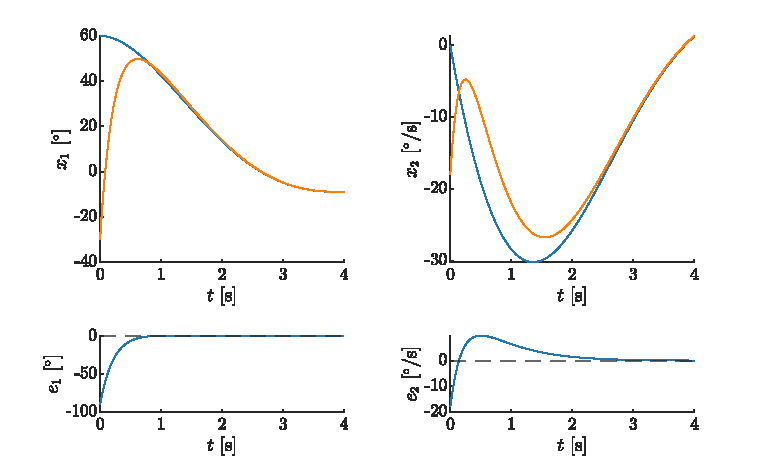
\includegraphics{figures/ex2_6.pdf}

The blue line is the true state and the orange line is estimated.

\subsection*{Code}
\subsubsection*{main system}
\begin{verbatim}
    u = @(t) 0;
    fx = @(t,x) [ x(2) ;...
                -x(2) - sin(x(1)) + u(t)];
    
    tspan = [0 4];
    y0 = [pi/3; 0];
    [t,y] = ode45(@(t,y) fx(t,y),tspan,y0);
\end{verbatim}

\subsubsection*{observer design}
\begin{verbatim}
    y_val = @(tt) interp1(t,y(:,1),tt,'spline');
    beta = 5;
    K = [beta; 1];
    fo = @(t,x) fx(t,x) + K * (y_val(t) - x(1));
    
    y0 = [-pi/6; -pi/10];
    [to,yo] = ode45(@(t,y) fo(t,y),tspan,y0);
\end{verbatim}
    
\subsubsection*{error signals}    
\begin{verbatim}
    yoo = interp1(t,y,to,'spline');
    err = (yo - yoo);
\end{verbatim}